Dette afsnit fokuserer på hvordan vi er kommet frem til designet af den endelige robot, som kan ses på \cref{robot:opbygning}, samt hvilke særlige problemstillinger, der ligger til grund for designet.

\begin{figure}
\centering
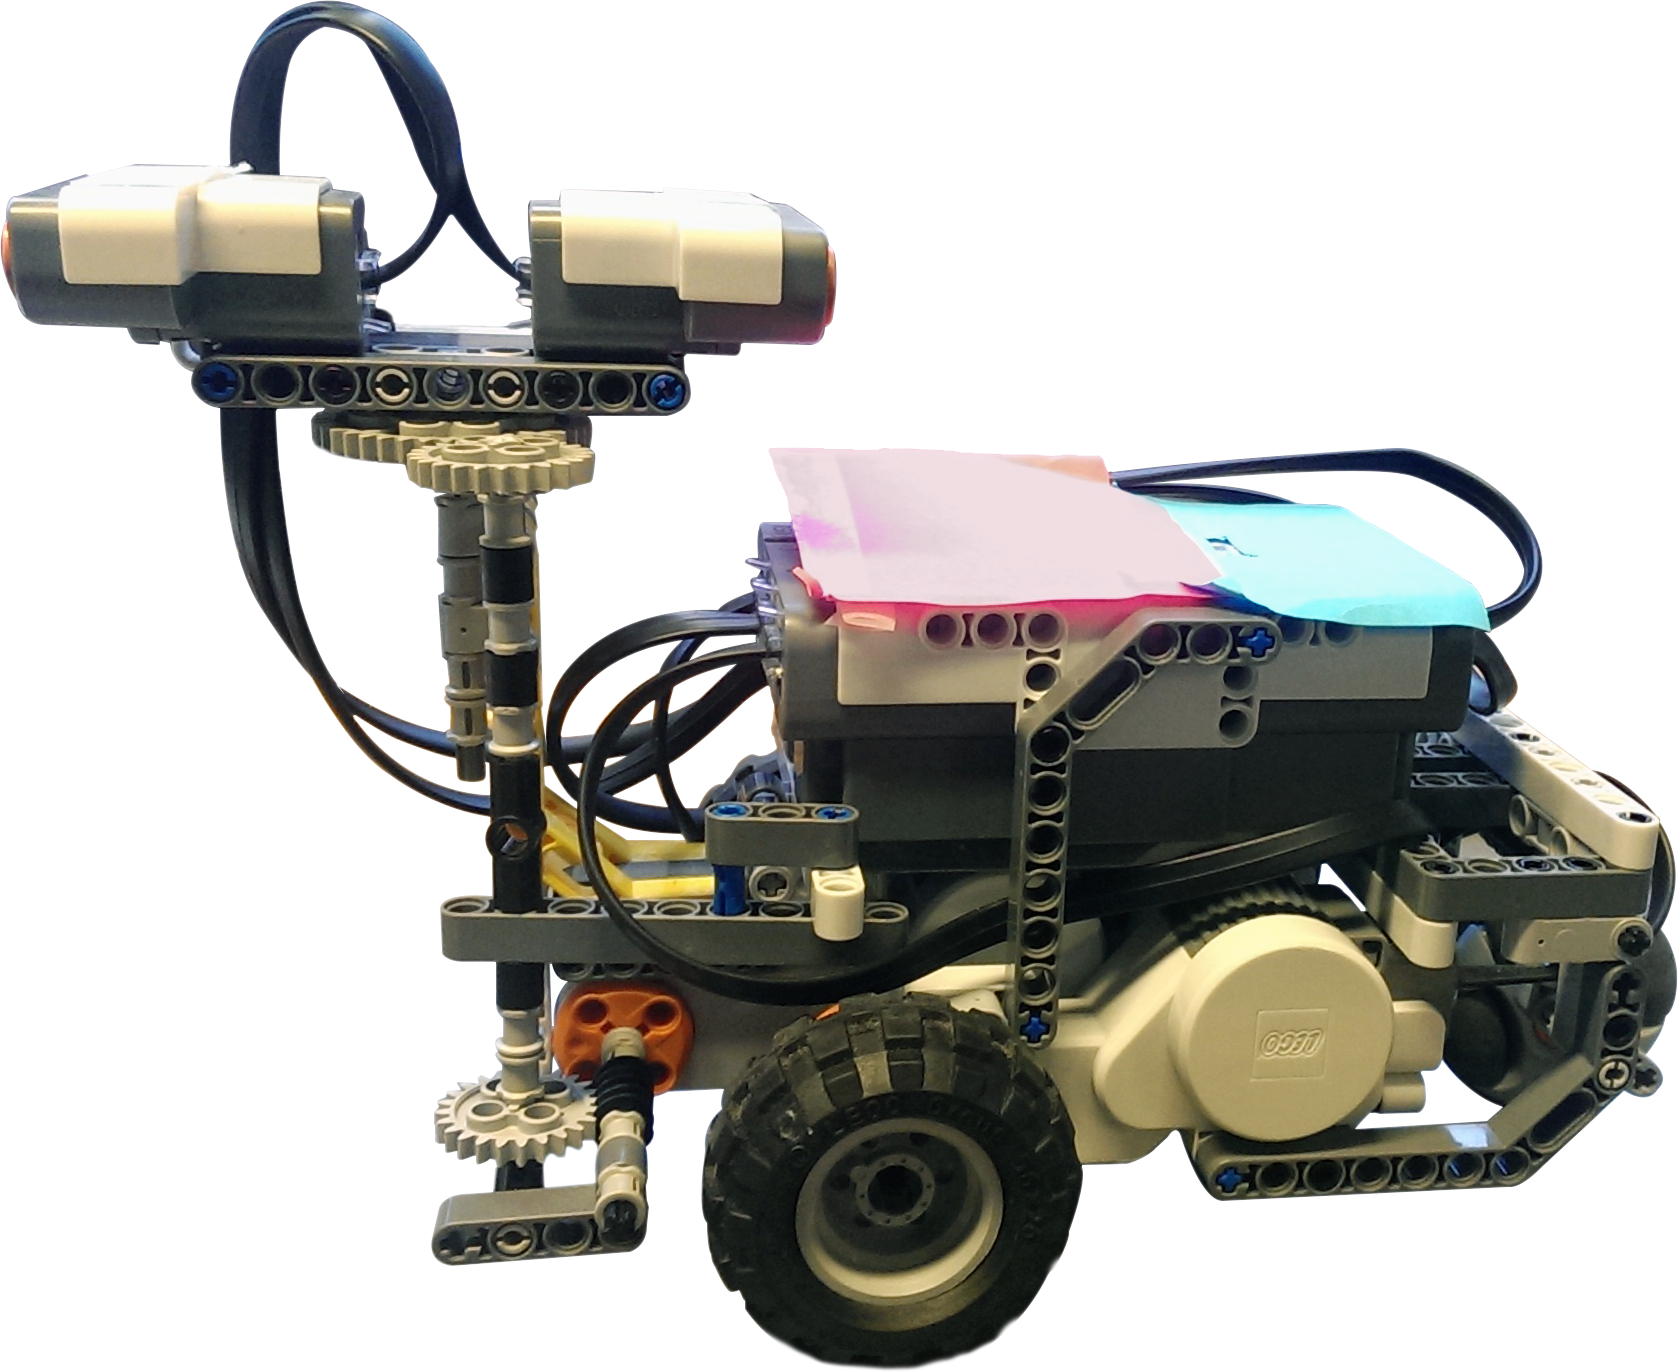
\includegraphics[width=0.6\textwidth]{whalle}
\caption{Endelige design af vores robot.}
\label{robot:opbygning}
\end{figure}

\section{Design krav}
\thilemann{Disse design krav gør sig ikke helt gældende længere. Vi antager bl.a. 90graders verden, hvorfor det ikke er et krav at sensoren kan rotere 360grader.}

\begin{itemize}
\item Den ultrasoniske sensor skal kunne styres med  minimum 1\degree~nøjagtighed, med en foreslået gearing på 1:4.
\item Sensoren(e) skal kunne foretage en 360\degree~måling.
%\item Sekundært indføres der en gearing af hjulene for bedre styring af robotten (nedgearing for højere moment).
\item Mere stabil opbygning for at mindske generelle usikkerheder (bl.a. sidder hjulene bedre fast på basen).
\end{itemize} 

\section{Endeligt design}
Udgangspunktet for det endelige design er baseret på ovenstående design krav sammen med andre idéer, der tilsammen skal øge præcisionen af robotten og gøre den mere driftsikker.

Den vigtigste faktor, når robotten bygges, er placeringen af de primære komponenter, såsom de ultrasoniske sensorer, der skal foretage afstandsmålinger og motoren, der skal skabe fremdrift.

\subsection{Kroppen}
Kroppen er den centrale komponent, hvor motorene, som styrer henholdsvis hjulene og rotation af sensorerne, er bygget på. 
Samtidig fungere den som det, der "holder robotten sammen".
Desuden er NXTen også en central del af denne konstruktion.
Placeringen af denne er primært i forhold til funktionelle behov, da der på fronten er knapper til at tænde/slukke og vælge indstillinger med.
Dens placering gør det også nemt at få adgang til dens porte for tilslutning af motor, sensor, opladning samt tilslutning af PC for opdatering af software med mere.

\subsection{Fremdrift}
Robotten er konstrueret med et \textit{aktivt} hjulsæt, der både giver fremdrift og styring.
Denne funktionalitet opnås ved, at hvert hjul (på hver side af robotten) har sin egen motor, således der kan angives både positiv og negativ fremdrift uafhængigt af hvert hjul.
Dette design gør det muligt at rotere robotten omkring sin egen akse for maksimal mobilitet -- selv på et begrænset område.
Foruden det forreste hjulsæt, er der bagerst på robotten monteret et 'baghjul', hvis eneste funktion er at balancere/stabilisere robotten.
Valget af et hjul til at udføre en sådan funktion er forholdsvis begrænset i \lego, hvorfor valget faldt på et "slæbehjul" med en masse ruller, der gør det muligt for hjulet at rotere i alle retninger.

\subsection{Sensorer}
Den egentlige funktion af robotten er at tage afstandsmålinger til objekter indenfor sensorernes rækkevidde.
Placeringen af sensorerne er derfor ikke kritisk, da de højst vil give en forskydelse af konstant faktor relativ til robottens midte fra deres placering i fronten.
Vigtigere er, at der er 360\degree~udsyn når de roterer, og at robotten ikke er i vejen for målingerne, hvilket er løst ved at montere sensorerne højere end resten af robotten.